\documentclass[12pt,letterpaper]{article} % script-article class - I like this better than article
\usepackage[margin=0.75in]{geometry}
\usepackage{graphicx}% Include figure files
\usepackage{dcolumn}% Align table columns on decimal point
\usepackage{bm}% bold math

\usepackage{helvet}
\usepackage{tikz}
\usepackage{tikz-3dplot}
\usepackage{mathtools}
\usepackage{amssymb,amsmath}
\usepackage{booktabs} % for much better looking tables
\usepackage{array} % for better arrays \left(eg matrices\right) in math
\usepackage{paralist} % very flexible & customisable lists \left(eg. enumerate/itemize, etc.\right)
\usepackage{verbatim} % adds environment for commenting out blocks of text & for better verbatim
%\usepackage[titles,subfigure]{tocloft} % Alter the style of the Table of Contents
%\usepackage{caption}
\usepackage{fixltx2e}% this might give you a warning; ignore it
%\usepackage{dblfloatfix}
\usepackage{float}
\usepackage{bbm}
\usepackage[space]{grffile}
\usepackage[section]{placeins}
\usepackage[justification=justified,singlelinecheck=false]{caption}

\captionsetup[figure]{labelformat=empty}

\newcommand{\bs}[1]{\bm{\mathrm{#1}}} % always use this custom command when you want to use boldface font in a math (equation, $__$ etc.) environment.
\newcommand{\switch}[0]{\mathbbm{1}\{y_k=k\}}
\renewcommand{\epsilon}{\varepsilon}

% the following are custom commands for quickly writing derivatives and partial derivatives
\newcommand{\ddt}[1]{\ensuremath{\dfrac{d#1}{dt}}}
\newcommand{\ddx}[1]{\ensuremath{\dfrac{d#1}{dx}}}
\newcommand{\ddy}[1]{\ensuremath{\dfrac{d#1}{dy}}}
\newcommand{\ddz}[1]{\ensuremath{\dfrac{d#1}{dz}}}

\newcommand{\pardt}[1]{\ensuremath{\dfrac{\partial#1}{\partial t}}}
\newcommand{\pardx}[1]{\ensuremath{\dfrac{\partial#1}{\partial x}}}
\newcommand{\pardy}[1]{\ensuremath{\dfrac{\partial#1}{\partial y}}}
\newcommand{\pardz}[1]{\ensuremath{\dfrac{\partial#1}{\partial z}}}

\newcommand{\pardtsq}[1]{\ensuremath{\dfrac{\partial^2#1}{\partial t^2}}}
\newcommand{\pardxsq}[1]{\ensuremath{\dfrac{\partial^2#1}{\partial x^2}}}
\newcommand{\pardysq}[1]{\ensuremath{\dfrac{\partial^2#1}{\partial y^2}}}
\newcommand{\pardzsq}[1]{\ensuremath{\dfrac{\partial^2#1}{\partial z^2}}}

\newcommand{\curl}[1]{\ensuremath{\nabla\times\bs{#1}}}

\newcommand{\figref}[1]{Fig.~\ref{#1}}
\newcommand{\tabref}[1]{Table~\ref{#1}}
\newcommand{\secref}[1]{Section~\ref{#1}}

%=====================

\title{\Large Assignment 1}
\author{\large Adriana Salcedo}
\date{\large \today}

\begin{document}
\maketitle

\section{Q1}

\subsection{}
 \begin{itemize}
 \item $y$ is a response for a single observation
  \item $\bs{x}$ is an N x d vector, in the case of a single observation (below) it is a 1 x d vector
  \item $\bs{\mu}_k$ is a 1 x d vector of the means of each feature for class k 
  \item $\bs{\sigma}$ is a d x 1 vector of the variances of each feature
  \item $\bs{\alpha}_k$ is a d x 1 vector of the prior for each class
 \end{itemize}


\begin{equation*}
 p(y=k | \bs{x},\bs{\mu}_k, \bs{\sigma}) = \frac{p(\bs{x}|y=k,\bs{\mu}_k,\bs{\sigma})p(y=k)}{p(\bs{x})} \\
\end{equation*}
 
\begin{equation*}
 =\frac{ \switch(2\pi\bs{\sigma}^T\bs{\sigma})^{-\frac{1}{2}}exp\{-\frac{1}{2\bs{\sigma}^T\bs{\sigma}}(\bs{x}-\bs{\mu}_k)(\bs{x}-\bs{\mu}_k)^T\}\bs{\alpha}_k}{\sum_{k=1}^K p(\bs{x} | \bs{\mu}_k, \bs{\sigma})\bs{\alpha}_k}
\end{equation*}

\begin{equation*}
 = \frac{ \switch(2\pi\bs{\sigma}^T\bs{\sigma})^{-\frac{1}{2}}exp\{-\frac{1}{2\bs{\sigma}^T\bs{\sigma}}(\bs{x}-\bs{\mu}_k)(\bs{x}-\bs{\mu}_k)^T\}\bs{\alpha}_k}{\sum_{k=1}^K (2\pi\bs{\sigma}^T\bs{\sigma})^{-\frac{1}{2}}exp\{-\frac{1}{2\bs{\sigma}^T\bs{\sigma}}(\bs{x}-\bs{\mu}_k)(\bs{x}-\bs{\mu}_k)^T\}\bs{\alpha}_k}
\end{equation*}

\subsection{}

For each class $k$
\begin{equation*}
\ell(\bs{\theta},D) = \prod^N_{n=1}\mathbbm{1}\{t_k=k\}p(\bs{x}_n|y_n=k,\bs{\mu}_k,\bs{\sigma})p(y=k)
\end{equation*}


\begin{equation*}
\prod^N_{n=1}\mathbbm{1}\{t_k=k\}(2\pi\bs{\sigma}^T\bs{\sigma})^{-\frac{1}{2}}exp\{-\frac{1}{2\bs{\sigma}^T\bs{\sigma}}(\bs{x}-\bs{\mu}_k)(\bs{x}-\bs{\mu}_k)^T\}\bs{\alpha}_k
\end{equation*}

Apply negative log

\begin{equation*}
= -\sum^N_n\switch\log{p(\bs{x}_n|y_n=k,\bs{\mu_k},\bs{\sigma})}-\switch\log{\alpha_k}
\end{equation*}

\begin{equation*}
 = -\sum^N_n\switch\log{(2\pi\bs{\sigma}^T\bs{\sigma})^{-\frac{1}{2}}} + \switch\frac{1}{2\bs{\sigma}^T\bs{\sigma}}(\bs{x}-\bs{\mu}_k)(\bs{x}-\bs{\mu}_k)^T-\switch\log{\bs{\alpha}_k}
\end{equation*}

\begin{equation*}
 =\sum^N_n\switch\frac{1}{2}\log{(2\pi\bs{\sigma}^T\bs{\sigma})}+ \sum^N_n\switch\frac{1}{2\bs{\sigma}^T\bs{\sigma}}(\bs{x}_n\bs{x}^T_n-2\bs{x}_n\bs{\mu}_k^T+\bs{\mu}_k\bs{\mu}_k^T)-\switch\log{\bs{\alpha}_k}
\end{equation*}

Taking the derivative with respect to $\mu_{ki}$ 

\begin{equation*}
  \sum^N_n\switch\frac{1}{2\bs{\sigma}^T\bs{\sigma}}(-2x_{ki}+2\mu_{ki})
\end{equation*}

Taking the derivative with respect to $\sigma_{ki}$ 

\begin{equation*}
=\sum^N_n\switch\frac{1}{2}\frac{1}{(2\pi\bs{\sigma}^T\bs{\sigma})}2\pi - \sum^N_n\switch\frac{1}{2}(\bs{\sigma}^T\bs{\sigma})^{-2}(\bs{x}_n\bs{x}^T_n-2\bs{x}_n\bs{\mu}_k^T+\bs{\mu}_k\bs{\mu}_k^T)
 \end{equation*}

\begin{equation*}
=\sum^N_n\switch\frac{1}{2}\frac{1}{(\bs{\sigma}^T\bs{\sigma})} - \sum^N_n\switch\frac{1}{2}(\bs{\sigma}^T\bs{\sigma})^{-2}(\bs{x}-\bs{\mu}_k)(\bs{x}-\bs{\mu}_k)^T
 \end{equation*}
 
\subsection{}

Setting the derivative with respect to $\mu_{ki}$  to zero

\begin{equation*}
 0 = \sum^N_n\switch\frac{1}{2\bs{\sigma}^T\bs{\sigma}}2x_{ki} + \sum^N_n\switch\frac{1}{2\bs{\sigma}^T\bs{\sigma}}2\mu_{ki}
\end{equation*}

\begin{equation*}
\sum^N_n\switch\frac{1}{\bs{\sigma}^T\bs{\sigma}}\mu_{ki} = \sum^N_n\switch\frac{1}{\bs{\sigma}^T\bs{\sigma}}x_{ki} 
\end{equation*}

\begin{equation*}
 \mu_{ki} = \frac{ \sum^N_n\switch{}x_{ki} }{\sum^N_n\switch}
\end{equation*}


For for feature i=1 to i=d, and for each class k =1 to k = k
\begin{equation*}
\bs{\mu}_k = \begin{bmatrix} \frac{ \sum^N_n\switch{}x_{k=1,i=1} }{\sum^N_n\switch} & \frac{ \sum^N_n\switch{}x_{k=1,i=2} }{\sum^N_n\switch} & ... & \frac{ \sum^N_n\switch{}x_{k=1, i=d} }{\sum^N_n\switch}\\  \frac{ \sum^N_n\switch{}x_{k=2,i=1} }{\sum^N_n\switch} & \frac{ \sum^N_n\switch{}x_{k=2,i=2} }{\sum^N_n\switch} & ... & \frac{ \sum^N_n\switch{}x_{k=2, i=d} }{\sum^N_n\switch} \\ ... \\  \frac{ \sum^N_n\switch{}x_{k=k,i=1} }{\sum^N_n\switch} & \frac{ \sum^N_n\switch{}x_{k=k,i=2} }{\sum^N_n\switch} & ... & \frac{ \sum^N_n\switch{}x_{k=k, i=d} }{\sum^N_n\switch} \end{bmatrix}
\end{equation*}

\clearpage
Setting the derivative with respect to $\sigma^2_{i}$  to zero

\begin{equation*}
0 =\sum^N_n\switch\frac{1}{2}\frac{1}{(\bs{\sigma}^T\bs{\sigma})} - \sum^N_n\switch\frac{1}{2}(\bs{\sigma}^T\bs{\sigma})^{-2}(\bs{x}-\bs{\mu}_k)(\bs{x}-\bs{\mu}_k)^T
 \end{equation*}
 
 
 \begin{equation*}
\sum^N_n\switch\frac{1}{2}\frac{1}{(\bs{\sigma}^T\bs{\sigma})}  = \sum^N_n\switch\frac{1}{2}\frac{1}{\bs{\sigma}^T\bs{\sigma}^2}(\bs{x}-\bs{\mu}_k)(\bs{x}-\bs{\mu}_k)^T
 \end{equation*}
 
  \begin{equation*}
\sum^N_n\switch  = \sum^N_n\switch\frac{1}{\bs{\sigma}^T\bs{\sigma}}(\bs{x}-\bs{\mu}_k)(\bs{x}-\bs{\mu}_k)^T
 \end{equation*}
 
   \begin{equation*}
\bs{\sigma}^T\bs{\sigma} = \frac{\sum^N_n\switch(\bs{x}-\bs{\mu}_k)(\bs{x}-\bs{\mu}_k)^T}{\sum^N_n\switch}
 \end{equation*}
 
 For each feature i
 \begin{equation*}
\sigma_i = \frac{\sum^N_n\switch(x_i-\mu_{ki})^2}{\sum^N_n\switch}
 \end{equation*}
 \
 \section{}
 
  \subsubsection{}
  \begin{figure}[!h]
  \centering
  \caption{}{ Means for each feature for each class}
   
\includegraphics[width=0.6\textwidth, trim={3in 0in 0in 0in},clip=true ]{q0_means.png}
\end{figure}
\FloatBarrier

\subsection{}
 \subsubsection{}
 K=1 train accuracy: 0.9998, test accuracy: 0.9685 \\
 K=15 train accuracy: 0.9596 test accuracy: 0.958\\
 
 \subsubsection {}
 
 I chose to break ties by randomly selecting a class from among the tied classes. I chose this approach as it gave each of the each of the classes tied for the most votes an equal chance of being selected, allowed the algorithm to use the same k for every point, did not exclude any test points, and always gave a class for each test point (ie there were no cases where a class was undefined). 
 
 \subsubsection{}
 
 The optimal k was 2. train accuracy: 0.9817, test accuracy: 0.9617
 
 \subsection{}
 
 MLE estimates for $\mu_k$ and $\Sigma_k$
 
 $\bs{x}_i$ is a d x 1 vector of the features for one observation and $\mu_{ki}$ is a d x 1 vector of the means of the features for class $k$. y is a N x 1 vector of responses for each observation indicating the class
 \begin{equation*}
  \ell(\bs{x},\bs{y}| \bs{\mu},\Sigma) = p(\bs{x}|y=k, \bs{\mu}_k,\Sigma)p(y=k)
 \end{equation*}
Applying the log

\begin{equation*}
 = \log{p(\bs{x}|y=k, \bs{\mu},\sigma)} + \log{p(y=k)}
 \end{equation*}

 \begin{equation*} 
  = \sum^N_{i=1}\switch{}\log{(2\pi)^{-\frac{d}{2}}|\Sigma_k|^{-\frac{1}{2}}}-\sum^N_{i=1}\switch{}\frac{1}{2}(\bs{x}_i-\bs{\mu}_{k})^T\Sigma_k^{-1}(\bs{x}_i -\bs{\mu}_{k}) + \log{\frac{1}{10}}
 \end{equation*}
 
  \begin{equation*} 
  = -\sum^N_{i=1}\switch{}\log{(2\pi)^{\frac{d}{2}}|\Sigma_k|^{\frac{1}{2}}}-\sum^N_{i=1}\switch{}\frac{1}{2}(\bs{x}_i-\bs{\mu}_{k})^T\Sigma_k^{-1}(\bs{x}_i -\bs{\mu}_{k}) + \log{\frac{1}{10}}
 \end{equation*}

taking the derivative w.r.t $\mu_{k}$ and setting it to zero

\begin{equation*} 
 0 = -\sum^N_{i=1}\switch\Sigma_k^{-1}\frac{1}{2}(-2\bs{x}_i + 2\bs{\mu}_{k})
\end{equation*}

\begin{equation*} 
 0 = \sum^N_{i=1}\switch\Sigma_k^{-1}\bs{x}_i - \sum^N_{i=1}\switch\Sigma_k^{-1} \bs{\mu}_{k}
\end{equation*}

\begin{equation*} 
 \sum^N_{i=1}\switch\Sigma_k^{-1}\bs{x}_i = \sum^N_{i=1}\switch\Sigma_k^{-1} \bs{\mu}_{k}
\end{equation*}

\begin{equation*} 
 \bs{\mu}_{k} =\frac{\sum^N_{i=1}\switch{}\bs{x}_i}{\sum^N_{i=1}\switch}
\end{equation*}

To solve for the covariance

\begin{equation*} 
 -\sum^N_{i=1}\switch{}\log{(2\pi)^{\frac{d}{2}}|\Sigma_k|^{\frac{1}{2}}}-\sum^N_{i=1}\switch{}\frac{1}{2}(x_i-\mu_{ki})^T\Sigma_k^{-1}(x_i -\mu_{ki}) + \log{\frac{1}{10}}
 \end{equation*}
 
 taking the derivative w.r.t $\Sigma^{-1}_{ki}$ and setting it to zero
 
 \begin{equation*} 
 0=-\sum^N_{i=1}\switch{}\frac{\partial\log{(2\pi)^{\frac{d}{2}}|\Sigma_k|^{\frac{1}{2}}}}{\partial\Sigma^{-1}_{k}}-\sum^N_{i=1}\switch{}\frac{1}{2}(\bs{x}_i-\bs{\mu}_k)(\bs{x}_i -\bs{\mu}_k)^T 
 \end{equation*}
 
 \begin{equation*} 
 0= \sum^N_{i=1}\switch(2\pi)^{-\frac{d}{2}}|\Sigma_k|^{-\frac{1}{2}}(2\pi)^{\frac{d}{2}}\frac{\partial|\Sigma_{k}^{-1}|^{-\frac{1}{2}}}{\partial\Sigma^{-1}_{k}} - \sum^N_{i=1}\switch{}\frac{1}{2}(\bs{x}_i-\bs{\mu}_k)(\bs{x}_i -\bs{\mu}_k)^T 
 \end{equation*}
 
  \begin{equation*} 
   0 = \sum^N_{i=1}\switch|\Sigma_k^{-1}|^{\frac{1}{2}}(-\frac{1}{2})|\Sigma_k^{-1}|^{-\frac{3}{2}}|\Sigma_{k}^{-1}|\Sigma_{k}^{T}- \sum^N_{i=1}\switch{}\frac{1}{2}(\bs{x}_i-\bs{\mu}_k)(\bs{x}_i -\bs{\mu}_k)^T 
  \end{equation*}

  \begin{equation*} 
   0 = \sum^N_{i=1}\switch(-\frac{1}{2})\Sigma_{k}- \sum^N_{i=1}\switch{}\frac{1}{2}(\bs{x}_i-\bs{\mu}_k)(\bs{x}_i -\bs{\mu}_k)^T 
  \end{equation*}

  \begin{equation*} 
   \Sigma_{k} = \frac{\switch \sum^N_{i=1}\switch{}(\bs{x}_i-\bs{\mu}_k)(\bs{x}_i -\bs{\mu}_k)^T }{\sum^N_{i=1}\switch}
  \end{equation*}
  
   \clearpage
  
  \subsubsection{}{}
  \begin{figure}[!h]
  \centering
  \caption{}{  Covariance matrix diagonals (variances) for each featutre}
   
\includegraphics[width=0.6\textwidth, trim={3in 0in 0in 0in},clip=true ]{q2_2_eta.png}
\end{figure}
\FloatBarrier

  \subsubsection{}
  Training average conditional log likelihood: -0.1264 \\
  Testing average conditional log likelihood: -0.1995\\
  \subsubsection{}
  Training accuracy: 0.98\\
  Testing accuracy: 0.97
 \subsection{}
 
  \addtocounter{subsubsection}{1}
 \subsubsection{}
 To get the MLE :
 
 \begin{equation*}
  \ell(\bs{x},\bs{y} | \bs{\eta}) = p(\bs{x} | \bs{\eta}_k, y_k=k)p(y_k = k)p{\bs{\eta}_k}
 \end{equation*}

Incorporate the prior on  $eta$ into the training data by adding a case of all positive and a case of all negative features to the training set.\\
For each class k: 

 \begin{equation*}
 =\prod^N_{i=1}\prod^d_{j=1}\switch(\eta_{jk})^{b_j}(1-\eta_{jk})^{(1-{b_j})}\frac{1}{10}
 \end{equation*}
Taking the log 


 \begin{equation*}
 =\sum^N_{i=1}\sum^d_{j=1}{b_j}\switch\big\{\log{(\eta_{jk})}+ (1-{b_j})\log{(1-\eta_{jk})} + \log{\frac{1}{10}}\big\}
 \end{equation*}

Taking the derivative w.r.t. $\eta_{jk}$ and setting it to zero
\begin{equation*}
0 = \sum^N_{i=1}\switch\big\{b_j\frac{1}{\eta_{jk}} + (1-{b_j})\frac{1}{(1-\eta_{jk})}(-1)\big\}
\end{equation*}

\begin{equation*}
0 = \sum^N_{i=1}\switch\big\{\frac{b_j}{\eta_{jk}} -\frac{1}{(1-\eta_{jk})} +  \frac{b_j}{(1-\eta_{jk})}\big\}
\end{equation*}

\begin{equation*}
0 = \sum^N_{i=1}\switch\big\{\frac{b_j}{\eta_{jk}} -\frac{1- b_j}{(1-\eta_{jk})}\big\}
\end{equation*}

\begin{equation*}
0 = \sum^N_{i=1}\switch\big\{{b_j}(1-\eta_{jk}) - \eta_{jk}(1-b_j)\big\}
\end{equation*}

\begin{equation*}
0 = \sum^N_{i=1}\switch\big\{b_j-b_j\eta_{jk} - \eta_{jk} + b_j\eta_{jk}\big\}
\end{equation*}

\begin{equation*}
\sum^N_{i=1}\switch\eta_{jk} = \sum^N_{i=1}\switch{}b_j
\end{equation*}


\begin{equation*}
\eta_{jk} = \frac{\sum^N_{i=1}\switch{}b_j}{\sum^N_{i=1}\switch}
\end{equation*}

\subsubsection{}
 \begin{figure}[!h]
  \centering
  \caption{}{  $eta$ for each class}
   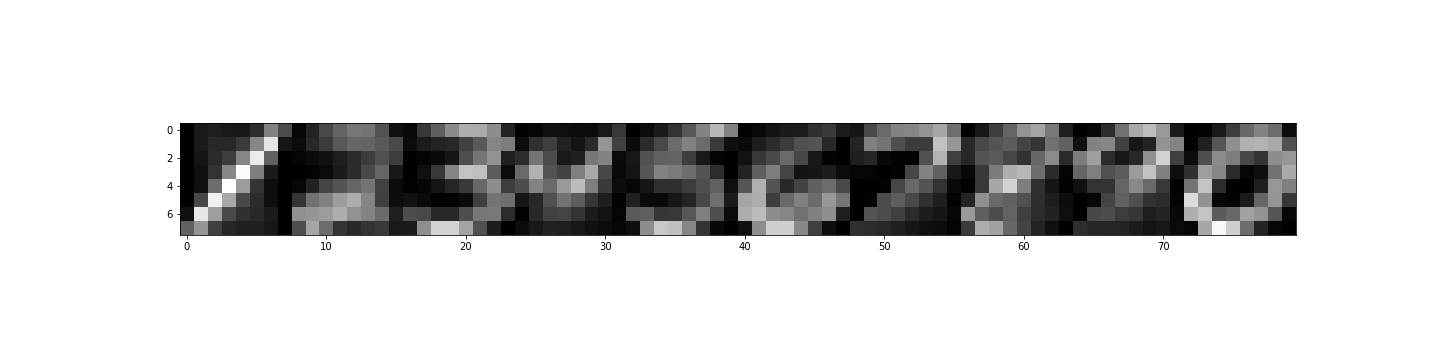
\includegraphics[width=0.6\textwidth, trim={3in 0in 0in 0in},clip=true ]{q2_3_eta.png}
\end{figure}
\FloatBarrier



\subsubsection{}
 \begin{figure}[!h]
  \centering
  \caption{}{ New data point }
   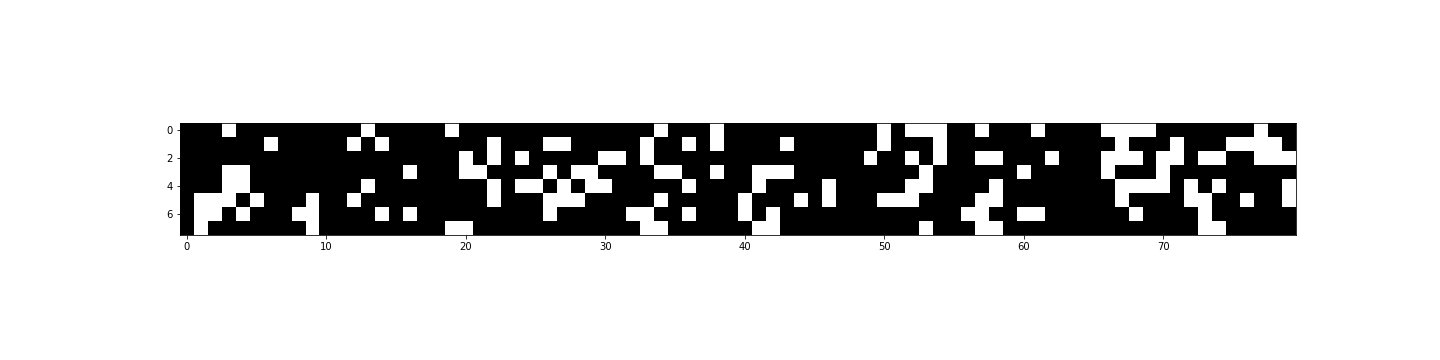
\includegraphics[width=0.6\textwidth, trim={3in 0in 0in 0in},clip=true ]{q2_3_new.png}
\end{figure}
\FloatBarrier

\subsubsection{}
 Training average conditional log likelihood: -0.9437 \\
  Testing average conditional log likelihood: -0.9872\\
  \subsubsection{}
  Training accuracy: 0.77\\
  Testing accuracy: 0.76
\end{document}